\chapter{Implementation}
\label{chap:impl}

In this chapter we describe the internal design of the tokenizer and provide
rationale for the choices behind it. We explore the problem of rough
tokenization more deeply as it posed one the biggest challenges in building the
system. Finally, we talk about the multi-threading tools which were used to
enable parallelism in the tokenizer.

\section{Overview of the System}
\label{sec:impl-overview}

The data flow between the various subsystems can be seen in
figure~\ref{fig:all-parts}.

\begin{figure}[ht]
  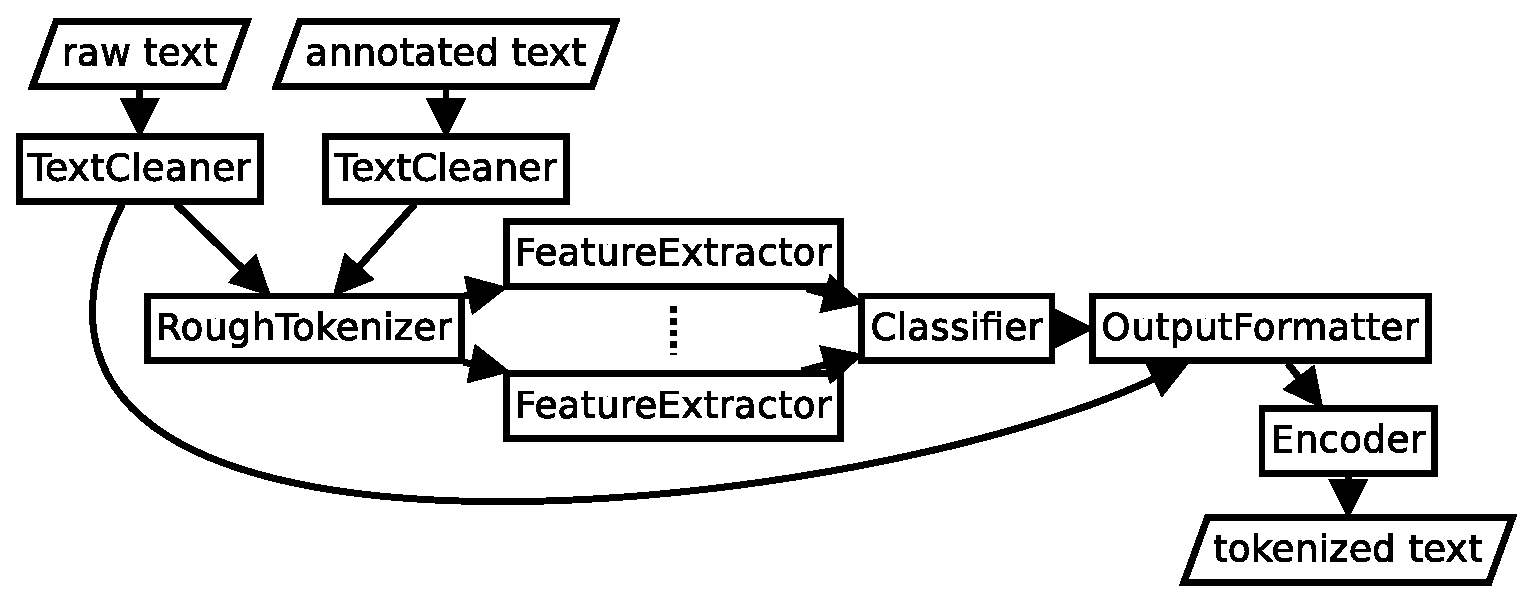
\includegraphics[width=\textwidth]{img/all-parts.eps}
  \caption{Data flow in the entire system}
  \label{fig:all-parts}
\end{figure}

\subsection{TextCleaner}

Any input which is read by the tokenizer is first processed with the
TextCleaner. This unit is responsible for decoding the stream of text and
optionally removing XML markup and expanding HTML entities and character
references. These changes to the input stream (referred to as cutouts in the
program) are conveyed to the OutputFormatter so that they can be undone in the
output. This allows the tokenizer to process XML marked up content as if it was
plaintext. The XML markup thus cannot be broken by and does not interfere with
the tokenization process.

\subsection{RoughTokenizer}

The RoughTokenizer's goal is to examine the cleaned input stream and identify
both unambiguous and ambiguous token and sentence boundaries. It does so by
splitting the text into what we call rough tokens. In the simplest case, rough
tokens are the whitespace delimited words of the text (the term word will be
used to mean a maximal subsequence of nonwhite characters). However, the user
can write regular expressions to define certain points within and between these
strings of nonwhite characters which may split them up into what end up being
the rough tokens. These user-defined points are called decision points and they
represent the ambiguous token/sentence boundaries.

There are three types of decision points. There is the MAY\_SPLIT which occurs
within words and signals a potential token boundary. The MAY\_BREAK\_SENTENCE
occurs before and after certain characters and marks a potential sentence
boundary. MAY\_SPLIT and MAY\_BREAK\_SENTENCE are the decision points which
split words into rough tokens. The third type of decision point is MAY\_JOIN
which occurs between words and turns the space between them from a token
boundary to a potential token boundary, making it possible for the two words to
join into a single token.

The rough tokenizer detects all decision points in the text and produces a
stream of discrete rough tokens annotated with information about surrounding
whitespace and decision points.

\subsection{FeatureExtractor}


